\chapter{Monolit, Modular Monolith, dan Microservices}
\label{ch:ch07}

\lstdefinestyle{ch07python}{
  language=Python,
  basicstyle=\ttfamily\scriptsize,
  keywordstyle=\color{blue}\bfseries,
  commentstyle=\color{gray}\itshape,
  stringstyle=\color{red},
  showstringspaces=false,
  breaklines=true,
  frame=lines,
  numbers=left,
  numberstyle=\tiny\color{gray},
  backgroundcolor=\color{lightgray!10},
  tabsize=2,
  captionpos=b
}

\section*{Tujuan Pembelajaran}
\begin{itemize}
  \item Membandingkan monolit, \textit{modular monolith}, dan \textit{microservices} dari sisi
        manfaat dan biayanya.
  \item Mendiagnosis sumber keterkaitan (\textit{coupling}) pada aplikasi yang ada.
  \item Menuliskan keputusan gaya arsitektur dalam format ADR.
\end{itemize}

\section{Pendahuluan}

Pada pertengahan 2026 sebuah vendor mempresentasikan ``SIMRS berbasis \textit{microservices}'' kepada
direksi Medikara Health. Janjinya menarik. Lima SIMRS (Sistem Informasi Manajemen Rumah Sakit) yang
berbeda versi akan diganti 32 layanan kecil yang dapat dirilis sendiri-sendiri, diskalakan
sendiri-sendiri, dan dikerjakan banyak tim sekaligus. Antrean panjang, rilis yang lambat, dan biaya
integrasi yang tinggi disebut akan selesai bersamaan. Direktur keuangan mengajukan pertanyaan
sederhana: bila \textit{microservices} sebagus itu, mengapa ada perusahaan yang justru kembali ke
monolit? Direktur teknologi informasi (TI) belum punya jawaban yang dapat dipertanggungjawabkan.

Pertanyaan itu adalah inti bab ini. \textit{Microservices} adalah satu gaya arsitektur, bukan
tujuan. Gaya ini menolong organisasi yang membutuhkan banyak tim bekerja mandiri pada bagian sistem
yang berbeda, tetapi menambah beban pada jaringan, data, pengujian, dan operasi. Di antara monolit
dan \textit{microservices} ada titik tengah, \textit{modular monolith}, yang sering terlewat dari
presentasi vendor. Tiga pilihan itu perlu dinilai melalui ketergantungan data, waktu, rilis,
dan makna. Inti SIMRS diarahkan menjadi modular monolith sebelum ekstraksi
layanan yang memang memerlukan distribusi.

\IfFileExists{../figures/ch07-diagram-konsep.png}{%
Gambar \ref{fig:ch07-tiga-kawasan} merangkum hubungan komponen dan konsep utama bab ini.
\begin{figure}[!htb]
  \centering
  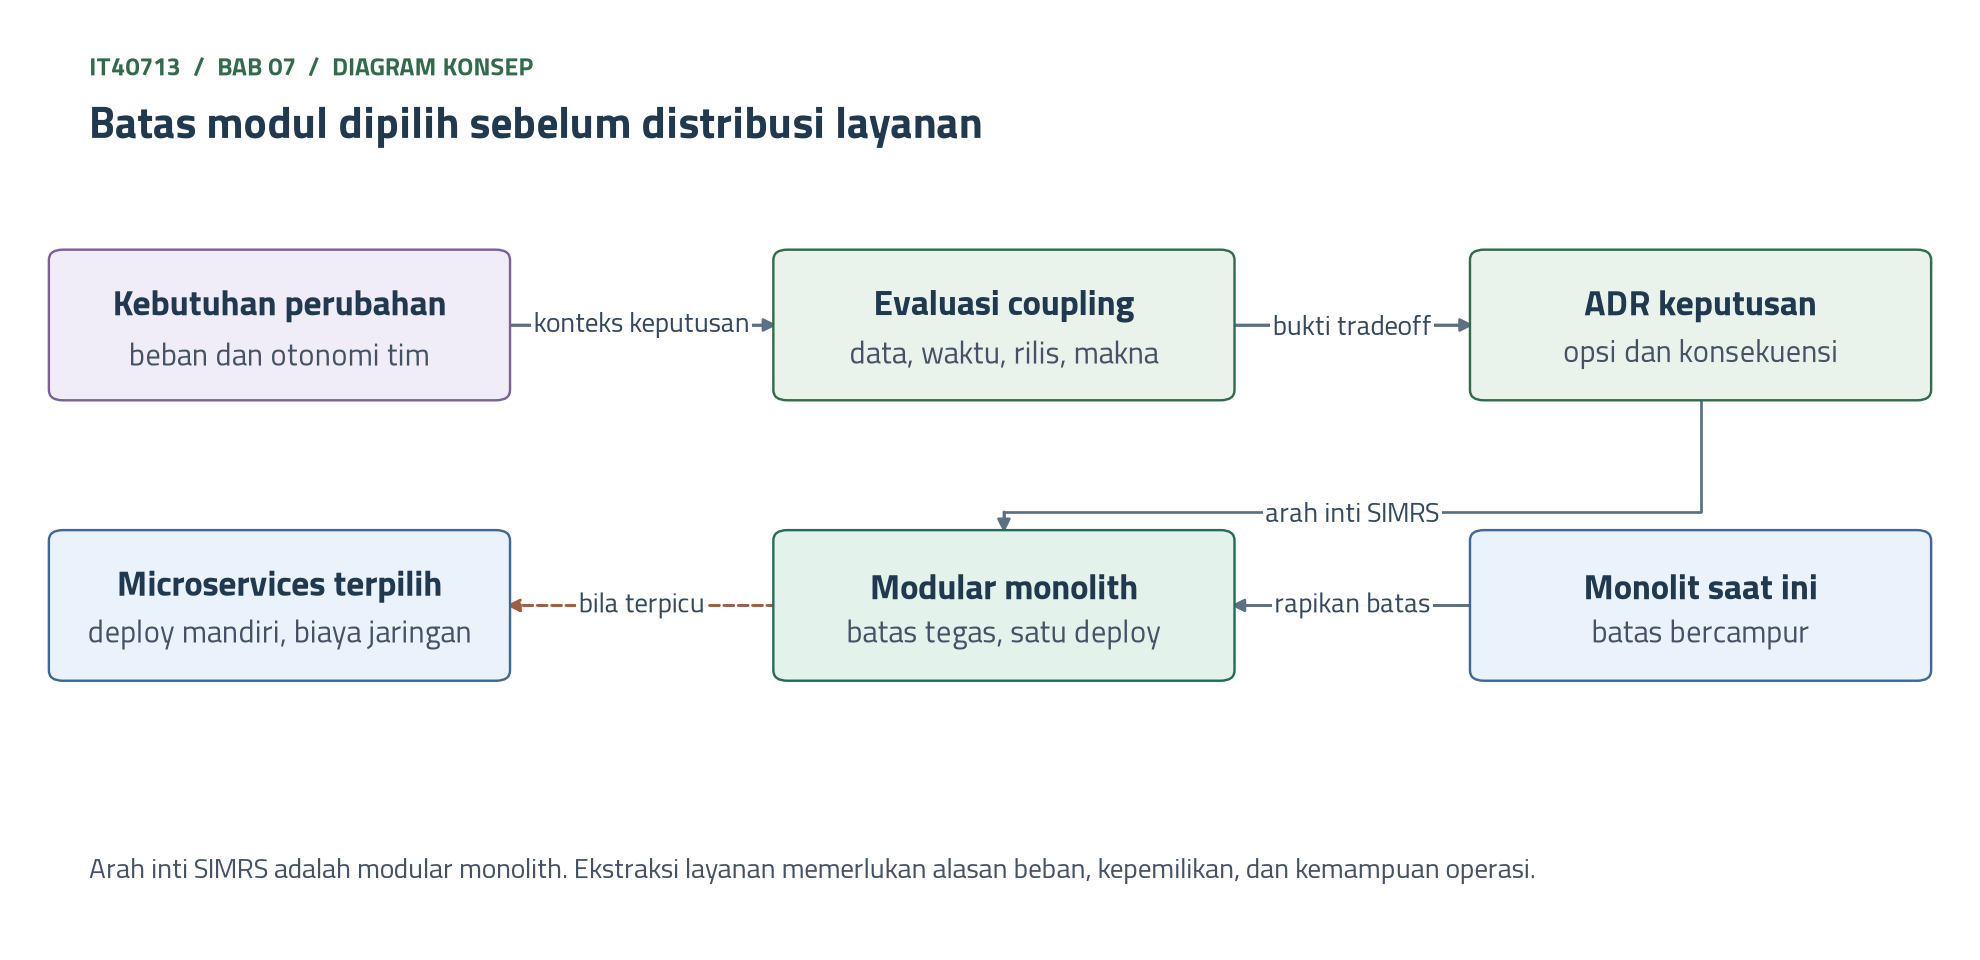
\includegraphics[width=\textwidth]{../figures/ch07-diagram-konsep.png}
  \caption{Batas modul dipilih sebelum distribusi layanan}
  \label{fig:ch07-tiga-kawasan}
\end{figure}
}{}

Bab ini disusun dalam lima langkah: ciri tiga gaya arsitektur, keterkaitan dan biaya sistem
terdistribusi, hukum Conway tentang hubungan struktur tim dengan struktur sistem, tanda-tanda
\textit{microservices} tidak tepat, serta Architecture Decision Record (ADR) sebagai catatan
keputusan. Rujukan utamanya adalah definisi \textit{microservices} dari Lewis dan Fowler
\cite{lewis-fowler2014}, buku Newman \cite{newman2021}, buku Richards dan Ford \cite{richards2025},
makalah Conway \cite{conway1968}, kajian Jamshidi dkk. \cite{jamshidi2018}, dan tulisan Nygard
tentang ADR \cite{c07-nygard2011}. Hasil bab ini adalah diagnosis arsitektur aplikasi inti dan ADR
gaya arsitektur, yang melengkapi tonggak capstone C2 untuk ditinjau menjelang Ujian Tengah Semester
(UTS).

\section{Tiga Gaya Arsitektur: Monolit, Modular Monolith, dan Microservices}
\label{sec:ch07-tiga-gaya}

Gaya arsitektur adalah cara menata bagian-bagian sistem dan hubungan antarbagiannya. Tiga gaya yang
dibahas di sini dibedakan oleh dua pertanyaan. Pertama, berapa unit yang dirilis secara terpisah?
Kedua, seberapa tegas batas antarbagian di dalam sistem dijaga? Jawaban atas dua pertanyaan itu
menentukan siapa yang dapat bekerja tanpa menunggu siapa, dan berapa biaya yang harus dibayar untuk
kemandirian tersebut.

\subsection{Monolit}

Monolit adalah sistem yang seluruh fungsinya dibangun, diuji, dan dirilis sebagai satu unit. Newman
memandang monolit sebagai satuan rilis: bila satu bagian berubah, seluruh sistem dirilis ulang
\cite{newman2021}. Umumnya semua bagian berjalan dalam satu proses dan berbagi satu basis data.
Monolit bukan kata yang buruk. Bagi tim kecil dan domain yang belum stabil, monolit adalah bentuk
yang paling sederhana dibangun, diuji, dan dioperasikan: satu tempat menyimpan kode, satu proses
rilis, satu tempat mencari kesalahan.

Masalah monolit muncul ketika ukurannya tumbuh tanpa batas internal yang dijaga. Setiap bagian boleh
memanggil bagian lain dan membaca tabel mana pun. Lama-kelamaan tidak ada yang berani mengubah satu
bagian tanpa menguji semuanya, dan jadwal rilis ditentukan oleh bagian yang paling lambat siap.

Analoginya seperti rumah makan dengan satu dapur. Selama rumah makan masih kecil, satu dapur membuat
semuanya cepat: juru masak saling membantu, bahan disimpan di satu lemari, dan pemilik mudah
mengawasi. Ketika rumah makan tumbuh menjadi seratus kursi dengan empat jenis masakan, semua juru
masak berdesakan di dapur yang sama, memakai kompor yang sama, dan saling menunggu. Dapurnya tidak
salah. Ukurannya yang tidak lagi cocok dengan cara kerja itu.

\subsection{Modular Monolith}

\textit{Modular monolith} tetap dirilis sebagai satu unit, tetapi isinya dibagi menjadi modul
dengan batas yang tegas. Setiap modul punya antarmuka publik, dan modul lain hanya boleh memakai
modul itu lewat antarmukanya. Data setiap modul dipisahkan, misalnya dalam skema basis data sendiri,
sehingga modul lain tidak membaca tabelnya secara langsung. Newman menempatkan \textit{modular
monolith} sebagai variasi monolit yang modulnya dapat dikerjakan terpisah walaupun tetap digabungkan
saat rilis \cite{newman2021}. Batas modul dijaga dengan aturan tertulis dan alat pemeriksa
otomatis, bukan sekadar kesepakatan lisan.

Analoginya seperti rumah sakit dalam satu kompleks bersayap. Ada sayap rawat jalan, sayap
laboratorium, dan sayap farmasi. Kompleksnya satu, atapnya satu, genset cadangannya satu. Namun
setiap sayap punya pintu, petugas, dan gudangnya sendiri. Petugas laboratorium tidak masuk ke gudang
farmasi untuk mengambil reagen. Ia mengajukan permintaan lewat loket farmasi.

\subsection{Microservices}

Lewis dan Fowler mendefinisikan \textit{microservices} sebagai pendekatan membangun satu aplikasi
sebagai sekumpulan layanan kecil. Setiap layanan berjalan dalam prosesnya sendiri, berkomunikasi
lewat mekanisme ringan seperti API (Application Programming Interface) berbasis web, dibangun
mengikuti kapabilitas bisnis, dan dirilis secara mandiri lewat otomasi \cite{lewis-fowler2014}.
Mereka mencatat sembilan ciri umum, antara lain penataan menurut kapabilitas bisnis, pengelolaan
data yang tersebar di setiap layanan, otomasi infrastruktur, dan rancangan yang siap menghadapi
kegagalan. Newman merumuskannya lebih ringkas: layanan yang dapat dirilis secara mandiri dan
dimodelkan di sekitar domain bisnis \cite{newman2021}. Kata kuncinya adalah dirilis secara
mandiri. Ukuran kecil bukan tujuan; kemandirian itulah tujuannya.

Analoginya seperti permukiman rumah kecil yang dihubungkan jalan. Setiap rumah dapat direnovasi
tanpa mengganggu tetangganya. Namun barang yang dulu cukup dipindah dari satu ruang ke ruang lain
kini harus diangkut lewat jalan. Jalan bisa macet, kendaraan bisa mogok, dan kawasan itu membutuhkan
petugas yang mengatur lalu lintas.

\subsection{Spektrum, Bukan Pilihan Biner}

Ketiga gaya ini sebaiknya dibaca sebagai titik pada satu spektrum, seperti diperlihatkan Gambar
\ref{fig:ch07-spektrum}. Makin ke kanan, kemandirian rilis dan penskalaan per bagian makin tinggi.
Biaya jaringan, data, pengujian, dan operasi juga ikut naik. Organisasi dapat berhenti di titik mana
pun, dan dapat bergeser bertahap, misalnya memisahkan satu modul menjadi layanan tersendiri ketika
data membuktikan perlunya.

\begin{figure}[!htb]
  \centering
  \begin{tikzpicture}[
  font=\scriptsize,
  panah/.style={-{Stealth[length=2mm]}, thick},
  modul/.style={draw, fill=white, rounded corners=1pt, minimum width=1.4cm,
    minimum height=0.45cm, font=\tiny, inner sep=1pt},
  layanan/.style={draw, fill=white, rounded corners=1pt, minimum width=1.15cm,
    minimum height=0.45cm, font=\tiny, inner sep=1pt},
  basis/.style={draw, cylinder, shape border rotate=90, aspect=0.25,
    fill=gray!15, minimum width=1.5cm, minimum height=0.6cm, font=\tiny,
    align=center, inner sep=1pt},
  tabung/.pic={
    \fill[gray!15] (-0.15,-0.2) rectangle (0.15,0.2);
    \fill[gray!15] (0,-0.2) ellipse [x radius=0.15, y radius=0.06];
    \draw (-0.15,0.2) -- (-0.15,-0.2)
      arc[start angle=180, end angle=360, x radius=0.15, y radius=0.06]
      -- (0.15,0.2);
    \draw[fill=gray!25] (0,0.2) ellipse [x radius=0.15, y radius=0.06];
  },
  ket/.style={font=\tiny, gray!60!black, align=center}
]
  % Panel 1: monolit, semua bagian saling menyentuh dan berbagi satu basis data.
  \draw[rounded corners, fill=blue!8] (0,0) rectangle (3.6,2.9);
  \node[font=\scriptsize\bfseries] at (1.8,3.2) {Monolit};
  \node[modul] (a1) at (0.95,2.4) {Pendaftaran};
  \node[modul] (a2) at (2.65,2.4) {Rekam medis};
  \node[modul] (a3) at (0.95,1.6) {Farmasi};
  \node[modul] (a4) at (2.65,1.6) {Penagihan};
  \node[basis] (adb) at (1.8,0.55) {satu basis data};
  \draw[gray!70!black] (a1) -- (a4);
  \draw[gray!70!black] (a2) -- (a3);
  \draw[gray!70!black] (a1) -- (a2);
  \draw[gray!70!black] (a3) -- (a4);
  \draw[gray!70!black] (a1) -- (a3);
  \draw[gray!70!black] (a2) -- (a4);
  \draw[gray!70!black] (a3.south) -- (adb.north west);
  \draw[gray!70!black] (a4.south) -- (adb.north east);
  \draw[gray!70!black] (a1.south west) to[bend right=25] (adb.west);
  \draw[gray!70!black] (a2.south east) to[bend left=25] (adb.east);
  \node[ket] at (1.8,-0.35) {satu unit rilis, bagian saling menyentuh};

  % Panel 2: modular monolith, satu unit rilis dengan batas modul yang ditegakkan.
  \draw[rounded corners, fill=orange!12] (4.2,0) rectangle (7.8,2.9);
  \node[font=\scriptsize\bfseries] at (6.0,3.2) {\textit{Modular monolith}};
  \node[modul, very thick] (b1) at (5.15,2.4) {Pendaftaran};
  \node[modul, very thick] (b2) at (6.85,2.4) {Rekam medis};
  \node[modul, very thick] (b3) at (5.15,1.6) {Farmasi};
  \node[modul, very thick] (b4) at (6.85,1.6) {Penagihan};
  \node[basis] (bdb) at (6.0,0.55) {skema per modul};
  \draw[panah, -{Stealth[length=1.5mm]}] (b2) -- (b1);
  \draw[panah, -{Stealth[length=1.5mm]}] (b4) -- (b3);
  \draw[gray!70!black] (b3.south) -- (bdb.north west);
  \draw[gray!70!black] (b4.south) -- (bdb.north east);
  \draw[gray!70!black] (b1.south west) to[bend right=25] (bdb.west);
  \draw[gray!70!black] (b2.south east) to[bend left=25] (bdb.east);
  \node[ket] at (6.0,-0.35) {satu unit rilis, batas modul ditegakkan};

  % Panel 3: microservices, banyak unit rilis yang berbicara lewat jaringan.
  \draw[rounded corners, fill=blue!8] (8.4,0) rectangle (12.0,2.9);
  \node[font=\scriptsize\bfseries] at (10.2,3.2) {\textit{Microservices}};
  \node[layanan] (c1) at (9.05,2.35) {Pendaftaran};
  \pic at (9.95,2.35) {tabung};
  \node[layanan] (c2) at (10.85,2.35) {Rekam medis};
  \pic at (11.72,2.35) {tabung};
  \node[layanan] (c3) at (9.05,0.7) {Farmasi};
  \pic at (9.95,0.7) {tabung};
  \node[layanan] (c4) at (10.85,0.7) {Penagihan};
  \pic at (11.72,0.7) {tabung};
  \draw[dashed, thick, gray!70!black] (8.6,1.52) -- (11.85,1.52);
  \node[font=\tiny, gray!60!black, fill=blue!8, inner sep=1pt] at (9.95,1.52)
    {jaringan};
  \draw[{Stealth[length=1.5mm]}-{Stealth[length=1.5mm]}] (c1.south) -- (9.05,1.52);
  \draw[{Stealth[length=1.5mm]}-{Stealth[length=1.5mm]}] (c2.south) -- (10.85,1.52);
  \draw[{Stealth[length=1.5mm]}-{Stealth[length=1.5mm]}] (c3.north) -- (9.05,1.52);
  \draw[{Stealth[length=1.5mm]}-{Stealth[length=1.5mm]}] (c4.north) -- (10.85,1.52);
  \node[ket] at (10.2,-0.35) {banyak unit rilis, data milik tiap layanan};

  % Dua sumbu: manfaat dan biaya naik bersama dari kiri ke kanan.
  \draw[panah, praditagreen] (0,-0.95) -- (12,-0.95)
    node[midway, above, font=\tiny, praditagreen] {kemandirian rilis dan
    penskalaan per bagian makin tinggi};
  \draw[panah, red!60!black] (0,-1.55) -- (12,-1.55)
    node[midway, above, font=\tiny, red!60!black] {biaya jaringan, data,
    pengujian, dan operasi makin tinggi};

  % Jebakan yang perlu dihindari.
  \node[draw, rounded corners, fill=red!22, align=center, font=\scriptsize,
    text width=7.6cm] at (6.0,-2.45)
    {\textbf{Jebakan: monolit terdistribusi}\\{\tiny\mdseries bagian dipisah
    lewat jaringan, tetapi tetap harus dirilis bersama:\\biaya
    \textit{microservices} ditanggung, manfaatnya tidak didapat}};
\end{tikzpicture}

  \caption{Tiga gaya arsitektur pada satu spektrum: manfaat dan biaya naik
           bersama, dengan monolit terdistribusi sebagai jebakan}
  \label{fig:ch07-spektrum}
\end{figure}

Ada satu titik yang harus dihindari. Newman menyebutnya monolit terdistribusi: sistem yang terdiri
atas beberapa layanan, tetapi seluruhnya harus dirilis bersama \cite{newman2021}. Organisasi yang
terjebak di sini membayar biaya jaringan seperti \textit{microservices}, tetapi tetap kaku seperti
monolit. Tabel \ref{tab:ch07-tiga-gaya} merangkum perbedaan ketiga gaya dari sisi yang biasa
ditanyakan manajemen.

\begin{table}[!htb]
  \centering
  \caption{Perbandingan monolit, \textit{modular monolith}, dan \textit{microservices}}
  \label{tab:ch07-tiga-gaya}
  \footnotesize
  \begin{tabularx}{\textwidth}{>{\raggedright\arraybackslash}p{2.3cm} >{\raggedright\arraybackslash}X >{\raggedright\arraybackslash}X >{\raggedright\arraybackslash}X}
    \hline
    \textbf{Aspek} & \textbf{Monolit} & \textbf{\textit{Modular monolith}} &
      \textbf{\textit{Microservices}} \\ \hline
    Unit rilis & Satu & Satu & Satu per layanan \\ \hline
    Batas antarbagian & Longgar, sering dilanggar & Tegas, dijaga alat pemeriksa & Tegas,
      dipisah jaringan \\ \hline
    Data & Satu basis data bersama & Satu basis data, skema per modul & Basis data per layanan \\
      \hline
    Komunikasi antarbagian & Pemanggilan di dalam proses & Pemanggilan di dalam proses lewat
      antarmuka modul & Pesan lewat jaringan \\ \hline
    Penskalaan & Seluruh sistem sekaligus & Seluruh sistem sekaligus & Per layanan \\ \hline
    Dampak kegagalan satu bagian & Dapat menghentikan seluruh sistem & Dapat menghentikan seluruh
      sistem & Terbatas, bila dirancang tahan gagal \\ \hline
    Syarat tim dan otomasi & Rendah & Sedang: disiplin menjaga batas & Tinggi: rilis otomatis,
      pemantauan, tim mandiri \\ \hline
    Cocok untuk & Tim kecil, domain belum jelas & Beberapa tim, satu jadwal rilis masih dapat
      diterima & Banyak tim yang perlu rilis dan skala mandiri \\ \hline
  \end{tabularx}
\end{table}

Dua contoh kasus nyata:
\begin{enumerate}
  \item Kode inti Shopify adalah salah satu basis kode Ruby on Rails terbesar, dikerjakan lebih
        dari seribu pengembang selama lebih dari sepuluh tahun. Tulisan teknik Shopify pada 2019
        menjelaskan pilihan untuk mengubahnya menjadi \textit{modular monolith}, bukan memecahnya
        menjadi \textit{microservices}, dengan alasan setiap panggilan lewat jaringan menambah
        waktu tunggu dan mengurangi keandalan. Sekitar 6.000 kelas program dipetakan ke komponen
        seperti pesanan, pengiriman, persediaan, dan penagihan, lalu pelanggaran batas
        antarkomponen dipantau dengan alat buatan sendiri \cite{c07-westeinde2019}.
  \item Segment, penyedia layanan pengolahan data pelanggan, pernah memecah sistem pengirimannya
        menjadi lebih dari 140 layanan, lalu menyatukannya kembali menjadi satu layanan
        \cite{noonan2018}. Kisah ini dibahas rinci di seksi \ref{sec:ch07-tidak-tepat}.
\end{enumerate}

\begin{kasus}[title={Kasus Medikara Health: SIMRS Monolitik sebagai Titik Awal}]
  SIMRS di lima rumah sakit Medikara Health berasal dari satu keluarga produk, dengan versi dari 3.9
  di Bandung sampai 5.2 di Jakarta. Setiap rumah sakit menyimpan salinan kode sendiri yang sudah
  dimodifikasi tim TI setempat. Setiap salinan adalah monolit: sembilan modul, yaitu pendaftaran,
  rekam medis, rawat inap, farmasi, laboratorium, radiologi, penagihan, klaim BPJS (Badan
  Penyelenggara Jaminan Sosial) Kesehatan, dan laporan, berjalan dalam satu aplikasi dan berbagi
  satu basis data.

  Misalkan basis data SIMRS Jakarta berisi sekitar 640 tabel, dan modul mana pun boleh membaca
  tabel mana pun. Rilis dilakukan tiga bulan sekali pada Sabtu malam dengan henti layanan sekitar
  empat jam. Setiap rilis harus menunggu modul yang paling lambat siap, sehingga perubahan tarif
  yang diminta bagian keuangan pada awal bulan rata-rata baru berlaku enam sampai sepuluh minggu
  kemudian.

  Diagnosis awal ini punya dua konsekuensi. Pertama, masalah Medikara tidak sesederhana ``monolit
  atau \textit{microservices}''. Masalahnya ada dua lapis: ada lima salinan, dan setiap salinan
  tidak punya batas internal. Kedua, pertanyaan yang lebih tepat untuk direksi adalah ``satu sistem
  atau lima, dan dengan batas atau tanpa batas''. Pertanyaan itu dijawab bertahap di seksi-seksi
  berikutnya, lalu dicatat dalam ADR.
\end{kasus}

\section{Coupling, Cohesion, dan Biaya Sistem Terdistribusi}
\label{sec:ch07-coupling}

Pertanyaan kemudian muncul: bagaimana mengetahui apakah batas antarbagian sebuah sistem sudah baik?
Jawabannya ada pada dua ukuran lama yang tetap dipakai sampai sekarang, yaitu \textit{coupling} dan
\textit{cohesion}. Keduanya juga menjelaskan mengapa memecah sistem lewat jaringan tidak otomatis
membuatnya lebih mudah diubah.

\subsection{Coupling dan Cohesion}

\textit{Coupling} adalah derajat ketergantungan antara dua bagian sistem. Makin tinggi
\textit{coupling}, makin besar kemungkinan perubahan di satu bagian memaksa perubahan di bagian
lain. \textit{Cohesion} adalah derajat keterkaitan isi di dalam satu bagian. Makin tinggi
\textit{cohesion}, makin besar kemungkinan hal-hal yang berubah bersama berada di tempat yang sama.
Kedua konsep ini diperkenalkan dalam kajian tentang rancangan program terstruktur oleh Stevens, Myers,
dan Constantine \cite{c07-stevens1974}. Arah yang dicari selalu sama: \textit{coupling} rendah
antarbagian dan \textit{cohesion} tinggi di dalam bagian. Bagi \textit{microservices}, ukuran ini
menentukan segalanya. Layanan yang terkait erat tidak dapat dirilis secara mandiri, sehingga
manfaat utama gaya ini hilang \cite{newman2021}.

Analoginya seperti panitia acara pernikahan dengan seksi konsumsi, seksi dekorasi, dan seksi acara.
Pada panitia yang baik, seksi konsumsi dapat mengganti menu tanpa rapat dengan seksi dekorasi
(\textit{coupling} rendah), dan semua urusan makanan memang ada di seksi konsumsi (\textit{cohesion}
tinggi). Pada panitia yang buruk, pemesanan katering dipegang seksi dekorasi karena kebetulan kenal
pemilik katering. Setiap perubahan menu kini membutuhkan dua seksi.

Dua hal pada \textit{coupling} sering tertukar. Pembagiannya begini. \textit{Coupling} yang tampak
adalah hubungan yang terlihat di diagram, misalnya modul A memanggil modul B. \textit{Coupling} yang
tersembunyi hanya terlihat dari riwayat, misalnya dua modul hampir selalu berubah dalam permintaan
perubahan yang sama walaupun di diagram tidak terhubung. Diagnosis yang baik membaca keduanya.

\subsection{Empat Jenis Coupling}

Untuk keperluan diagnosis, bab ini memakai empat jenis \textit{coupling} yang mudah dikenali di
lapangan, baik oleh anggota teknis maupun non-teknis. Tabel \ref{tab:ch07-jenis-coupling}
merangkumnya beserta tanda-tandanya.

\begin{table}[!htb]
  \centering
  \caption{Empat jenis \textit{coupling} dan tandanya di lapangan}
  \label{tab:ch07-jenis-coupling}
  \footnotesize
  \begin{tabularx}{\textwidth}{>{\raggedright\arraybackslash}p{1.7cm} >{\raggedright\arraybackslash}X >{\raggedright\arraybackslash}X >{\raggedright\arraybackslash}X}
    \hline
    \textbf{Jenis} & \textbf{Arti} & \textbf{Tanda di lapangan} & \textbf{Contoh di Medikara} \\
      \hline
    Data & Dua bagian membaca atau menulis data yang sama & Satu perubahan kolom memaksa banyak
      bagian diuji ulang & Aplikasi apotek membaca tabel SIMRS secara langsung (Bab 4) \\ \hline
    Waktu & Satu bagian hanya dapat bekerja bila bagian lain menyala pada saat yang sama & Gangguan
      satu sistem ikut menghentikan sistem lain & Pemesanan janji temu di Medikara+ berhenti saat
      SIMRS dipelihara \\ \hline
    Rilis & Dua bagian harus dirilis bersama & Jadwal rilis menunggu tim lain & Perubahan tarif
      menunggu rilis modul klaim \\ \hline
    Makna & Dua bagian bergantung pada arti dan aturan yang sama & Arti satu kode berubah, bagian
      lain salah tafsir tanpa ada pesan kesalahan & Status ``pulang'' dipakai rawat inap dan
      penagihan dengan arti berbeda \\ \hline
  \end{tabularx}
\end{table}

\textit{Coupling} makna paling sulit ditemukan karena tidak menimbulkan \textit{error}. Sistem
berjalan normal, tetapi angkanya salah. Jenis ini berkaitan langsung dengan \textit{bounded
context} pada Bab 6: satu istilah yang dipakai lintas konteks tanpa kesepakatan arti adalah sumber
\textit{coupling} makna. Jenis data paling mudah dilihat dan paling sering ditemui pada monolit.
Gambar \ref{fig:ch07-coupling-data} membandingkan kondisi SIMRS sekarang, ketika semua modul berbagi
tabel yang sama, dengan kondisi target ketika setiap modul memiliki datanya sendiri.

\begin{figure}[!htb]
  \centering
  \begin{tikzpicture}[
  font=\scriptsize,
  panah/.style={-{Stealth[length=2mm]}, thick},
  modul/.style={draw, rounded corners, fill=blue!8, minimum width=1.9cm,
    minimum height=0.6cm, text height=1.6ex, text depth=0.4ex},
  luar/.style={draw, rounded corners, fill=gray!35, minimum width=1.9cm,
    minimum height=0.6cm, align=center},
  basis/.style={draw, cylinder, shape border rotate=90, aspect=0.22,
    fill=gray!15, minimum width=1.6cm, minimum height=0.7cm, font=\tiny,
    align=center},
  akses/.style={{Stealth[length=1.5mm]}-{Stealth[length=1.5mm]}, gray!60!black},
  tersembunyi/.style={-{Stealth[length=2mm]}, thick, dashed, red!70!black},
  ket/.style={font=\tiny, gray!60!black}
]
  % Bagian atas: kondisi sekarang, semua modul membaca dan menulis tabel yang sama.
  \node[anchor=west, font=\scriptsize\bfseries] at (-0.2,7.15)
    {Sekarang: semua bagian berbagi tabel yang sama};
  \node[modul] (p1) at (1.0,6.3) {Pendaftaran};
  \node[modul] (p2) at (3.5,6.3) {Rekam medis};
  \node[modul] (p3) at (6.0,6.3) {Farmasi};
  \node[modul] (p4) at (8.5,6.3) {Penagihan};
  \node[modul] (p5) at (11.0,6.3) {Klaim BPJS};
  \node[basis, minimum width=3.6cm, minimum height=1.0cm] (db) at (6.0,4.55)
    {\textbf{Basis data SIMRS}\\tabel pasien, kunjungan,\\resep, tagihan};
  \draw[akses] (p1.south) -- (db.north west);
  \draw[akses] (p2.south) -- (db.north);
  \draw[akses] (p3.south) -- (db.north);
  \draw[akses] (p4.south) -- (db.north);
  \draw[akses] (p5.south) -- (db.north east);
  \node[luar] (apotek) at (11.0,4.55) {Aplikasi apotek\\
    {\tiny\mdseries di luar SIMRS}};
  \draw[tersembunyi] (apotek.west) -- node[ket, above, red!70!black]
    {baca langsung} (db.east);
  \node[draw, rounded corners, fill=red!22, text width=3.0cm, align=center,
    font=\tiny] at (1.4,4.55)
    {Satu kolom di tabel pasien diubah: enam bagian ikut diuji dan dirilis
    bersama};

  % Garis pemisah.
  \draw[dashed, gray] (-0.2,3.45) -- (12.2,3.45);

  % Bagian bawah: kondisi target, tiap modul memiliki datanya sendiri.
  \node[anchor=west, font=\scriptsize\bfseries] at (-0.2,3.0)
    {Target: tiap modul memiliki datanya, modul lain bertanya lewat antarmuka};
  \node[modul, fill=green!10] (q1) at (1.0,2.15) {Pendaftaran};
  \node[modul, fill=green!10] (q2) at (3.5,2.15) {Rekam medis};
  \node[modul, fill=green!10] (q3) at (6.0,2.15) {Farmasi};
  \node[modul, fill=green!10] (q4) at (8.5,2.15) {Penagihan};
  \node[modul, fill=green!10] (q5) at (11.0,2.15) {Klaim BPJS};
  \node[basis] (d1) at (1.0,0.85) {data\\pendaftaran};
  \node[basis] (d2) at (3.5,0.85) {data\\klinis};
  \node[basis] (d3) at (6.0,0.85) {data\\resep};
  \node[basis] (d4) at (8.5,0.85) {data\\tagihan};
  \node[basis] (d5) at (11.0,0.85) {data\\klaim};
  \foreach \nomor in {1,...,5} {
    \draw[akses] (q\nomor.south) -- (d\nomor.north);
  }
  \draw[panah] (q2) -- (q1);
  \draw[panah] (q3) -- (q2);
  \draw[panah] (q4) -- (q3);
  \draw[panah] (q5) -- (q4);
  \node[ket] at (2.25,2.62) {antarmuka};
  \node[ket] at (4.75,2.62) {antarmuka};
  \node[ket] at (7.25,2.62) {antarmuka};
  \node[ket] at (9.75,2.62) {antarmuka};
  \node[draw, rounded corners, fill=green!10, text width=9.0cm, align=center,
    font=\tiny] at (6.0,-0.2)
    {Satu kolom data pendaftaran diubah: cukup modul pendaftaran yang diuji,
    selama antarmukanya tetap};
\end{tikzpicture}

  \caption{\textit{Coupling} data: berbagi tabel membuat satu perubahan kecil
           merambat ke banyak bagian, sedangkan kepemilikan data menahannya di
           satu modul}
  \label{fig:ch07-coupling-data}
\end{figure}

Dua contoh dari Medikara Health:
\begin{enumerate}
  \item Misalkan kolom nomor telepon di tabel pasien SIMRS Jakarta diubah dari satu nomor menjadi
        daftar nomor. Enam bagian membaca tabel itu, termasuk aplikasi apotek di luar SIMRS.
        Dengan pengujian manual sekitar dua hari kerja per bagian, satu perubahan kecil
        membutuhkan 12 hari kerja pengujian.
  \item Medikara+ memesan janji temu dengan memanggil SIMRS secara langsung. Ketika SIMRS Bogor
        menjalani pemeliharaan malam selama empat jam, pemesanan janji temu untuk rumah sakit
        Bogor ikut berhenti selama empat jam, walaupun Medikara+ sendiri sehat. Ini contoh
        \textit{coupling} waktu.
\end{enumerate}

\subsection{Fallacies of Distributed Computing}

Ketika bagian sistem dipisah lewat jaringan, panggilan yang dulu terjadi di dalam satu proses
berubah menjadi pesan yang melintasi jaringan. Para insinyur Sun Microsystems pada 1990-an merangkum
delapan asumsi keliru yang sering dipegang perancang sistem terdistribusi. Daftar ini dikenal
sebagai \textit{fallacies of distributed computing}, dan Richards serta Ford memakainya sebagai
titik awal setiap pembahasan gaya arsitektur terdistribusi \cite{richards2025}. Tabel
\ref{tab:ch07-fallacies} menerjemahkan kedelapannya ke akibat yang dirasakan organisasi.

Analoginya seperti memindahkan rapat dari satu ruangan ke surat-menyurat antarkota. Dalam satu
ruangan, pertanyaan langsung dijawab. Lewat pos, surat dapat terlambat, hilang, atau dibuka orang di
jalan. Ongkos kirimnya tidak nol, dan alamat penerimanya dapat pindah tanpa pemberitahuan.

\begin{table}[!htb]
  \centering
  \caption{Delapan \textit{fallacies of distributed computing} dan akibatnya bagi
           organisasi, diolah dari Richards dan Ford \cite{richards2025}}
  \label{tab:ch07-fallacies}
  \footnotesize
  \begin{tabularx}{\textwidth}{>{\raggedright\arraybackslash}p{3.0cm} >{\raggedright\arraybackslash}X >{\raggedright\arraybackslash}X}
    \hline
    \textbf{Asumsi keliru} & \textbf{Kenyataan} & \textbf{Akibat bagi organisasi} \\ \hline
    Jaringan selalu andal & Pesan dapat hilang atau terputus & Setiap panggilan perlu pengulangan
      dan penanganan gagal \\ \hline
    Latensi nol & Setiap panggilan membutuhkan waktu & Permintaan yang melewati banyak layanan
      terasa lambat bagi pasien \\ \hline
    \textit{Bandwidth} tidak terbatas & Kapasitas jaringan terbatas & Berkas besar seperti citra
      radiologi membebani jaringan antarlokasi \\ \hline
    Jaringan aman & Setiap jalur dapat disadap & Setiap layanan perlu otentikasi dan enkripsi,
      menambah kerja kepatuhan \\ \hline
    Topologi tidak berubah & Alamat dan jalur berpindah & Alamat layanan harus dicari secara
      dinamis, bukan ditulis di kode \\ \hline
    Hanya ada satu administrator & Banyak tim dan vendor terlibat & Perubahan perlu koordinasi
      lintas tim dan lintas kontrak \\ \hline
    Biaya transpor nol & Transfer dan pengolahan pesan berbiaya & Tagihan transfer data dan
      tenaga pemantauan naik \\ \hline
    Jaringan seragam & Perangkat dan protokol beragam & Pengujian harus mencakup banyak kombinasi
      lingkungan \\ \hline
  \end{tabularx}
\end{table}

Pemisahan lewat jaringan membawa empat jenis biaya tambahan. Pertama, biaya jaringan: setiap
panggilan dapat lambat atau gagal, sehingga perlu batas waktu, pengulangan, dan rancangan tahan gagal
yang dibahas di Bab 12. Kedua, biaya data: tabel tidak lagi dapat digabung dalam satu
\textit{query}, dan perubahan yang menyentuh beberapa layanan memerlukan pola khusus seperti saga
pada Bab 10. Ketiga, biaya pengujian: setiap layanan diuji sendiri, lalu kesepakatan antarlayanan
juga harus diuji. Keempat, biaya operasi: setiap layanan butuh jalur rilis, pemantauan, dan pemilik
yang siap dihubungi ketika terjadi gangguan, seperti dibahas di Bab 11 dan Bab 13.

Biaya pertama dapat dihitung. Misalkan satu pemesanan janji temu di Medikara+ melewati enam layanan
secara berurutan, dan setiap layanan tersedia 99,9 persen dari waktu. Ketersediaan rangkaian itu
adalah $0{,}999^{6} \approx 0{,}994$, atau sekitar 99,4 persen. Dalam sebulan berisi 30 hari, satu
layanan dengan ketersediaan 99,9 persen boleh tidak tersedia sekitar 43 menit. Rangkaian enam
layanan boleh tidak tersedia sekitar 4 jam 19 menit, enam kali lebih lama. Angka ini menjelaskan
mengapa \textit{microservices} menuntut rancangan tahan gagal sejak awal.

\begin{kasus}[title={Kasus Medikara Health: Diagnosis Coupling SIMRS Jakarta}]
  Misalkan tim transformasi mengumpulkan dua jenis data dari SIMRS Jakarta. Data pertama adalah 40
  permintaan perubahan pada Januari sampai Maret 2025, masing-masing dengan daftar modul yang
  diubah. Data kedua adalah 63 catatan gangguan sepanjang 2025. Anggota non-teknis mewawancarai
  bagian peminta untuk mengetahui dampak bisnis setiap modul. Hasilnya ada di Tabel
  \ref{tab:ch07-diagnosis-simrs}.

  Hasil ini punya tiga konsekuensi. Pertama, 30 dari 40 perubahan (75 persen) menyentuh lebih dari
  satu modul. Batas modul yang ada sekarang tidak mengikuti cara bisnis berubah. Kedua, modul klaim
  BPJS dan penagihan berubah bersama 10 kali dari 13 perubahan modul klaim, dengan derajat
  keterkaitan 67 persen. Keduanya kandidat kuat untuk disatukan dalam satu modul dan dipegang satu
  tim, bukan dipisah menjadi dua layanan. Ketiga, modul klaim menyumbang 22 dari 63 gangguan
  (sekitar 35 persen), sehingga modul inilah yang paling mendesak dirapikan. Rincian perhitungannya
  tersedia di \berkas{sources/chapter07/lembar-diagnosis-coupling.xlsx}.
\end{kasus}

\begin{table}[!htb]
  \centering
  \caption{Diagnosis SIMRS Jakarta: perubahan Januari sampai Maret 2025 dan
           gangguan sepanjang 2025 (angka rekaan)}
  \label{tab:ch07-diagnosis-simrs}
  \footnotesize
  \begin{tabularx}{\textwidth}{>{\raggedright\arraybackslash}p{2.0cm} r r >{\raggedright\arraybackslash}X >{\raggedright\arraybackslash}X}
    \hline
    \textbf{Modul} & \textbf{Perubahan} & \textbf{Gangguan} & \textbf{Pasangan paling erat
      (kali berubah bersama)} & \textbf{Dampak bisnis bila terganggu} \\ \hline
    Pendaftaran & 9 & 9 & Rekam medis (5) & Antrean pagi memanjang \\ \hline
    Rekam medis & 13 & 6 & Pendaftaran (5) & Dokter kembali menulis di kertas \\ \hline
    Rawat inap & 4 & 3 & Tidak ada yang menonjol & Penempatan pasien lambat \\ \hline
    Farmasi & 6 & 5 & Tidak ada yang menonjol & Pasien menunggu obat \\ \hline
    Laboratorium & 5 & 4 & Rekam medis (4) & Hasil terlambat sampai ke dokter \\ \hline
    Radiologi & 2 & 2 & Tidak ada yang menonjol & Jadwal pemeriksaan bergeser \\ \hline
    Penagihan & 17 & 11 & Klaim BPJS (10) & Pasien tertahan di kasir \\ \hline
    Klaim BPJS & 13 & 22 & Penagihan (10) & Klaim tertunda, arus kas terganggu \\ \hline
    Laporan & 7 & 1 & Klaim BPJS (3) & Rapat direksi tanpa angka terbaru \\ \hline
    \textbf{Jumlah} & \textbf{76} & \textbf{63} & 76 sentuhan modul berasal dari 40 permintaan;
      30 permintaan (75 persen) menyentuh lebih dari satu modul & \\ \hline
  \end{tabularx}
\end{table}

\begin{pendalaman}[title={Pendalaman Teknis (opsional): Mengukur Coupling pada Basis Kode}]
  \textit{Coupling} yang tampak diukur dari dependensi statis di kode. Alat analisis dependensi
  seperti \texttt{jdeps} untuk Java atau \texttt{pydeps} untuk Python menghasilkan graf modul
  yang saling memanggil. Dari graf itu dihitung dua angka untuk setiap modul: berapa modul lain
  yang bergantung padanya (\textit{afferent coupling}, $C_a$) dan berapa modul lain yang ia
  butuhkan (\textit{efferent coupling}, $C_e$). Martin menggabungkan keduanya menjadi
  \textit{instability} $I = C_e / (C_a + C_e)$. Nilai mendekati 0 menandakan modul yang banyak
  diandalkan dan sebaiknya jarang berubah, sedangkan nilai mendekati 1 menandakan modul yang
  bebas berubah \cite{c07-martin2003}. Misalkan modul penagihan dipakai empat modul dan memakai
  dua modul. Nilainya $I = 2/6 \approx 0{,}33$, sehingga perubahan antarmukanya harus hati-hati.

  \textit{Coupling} yang tersembunyi diukur dari riwayat perubahan. Listing
  \ref{lst:ch07-hitung-coupling} memperlihatkan inti skrip yang menghitung pasangan modul yang
  sering berubah bersama. Derajat keterkaitan dihitung terhadap rata-rata jumlah perubahan kedua
  modul, agar modul yang sangat sering berubah tidak membuat semua pasangannya tampak erat. Pada
  berkas contoh \berkas{sources/chapter07/contoh-riwayat-perubahan.csv}, skrip menemukan 30 dari 40
  perubahan menyentuh lebih dari satu modul, dan pasangan klaim BPJS dengan penagihan berubah
  bersama 10 kali dengan derajat 67 persen, sama dengan Tabel \ref{tab:ch07-diagnosis-simrs}.

\begin{lstlisting}[style=ch07python, caption={Inti penghitung keterkaitan perubahan, tersedia di \berkas{sources/chapter07/hitung-coupling.py}}, label={lst:ch07-hitung-coupling}]
def hitung_keterkaitan(daftar_perubahan):
  """Menghitung jumlah perubahan per modul dan per pasangan modul.

  Pasangan diurutkan menurut abjad agar (a, b) dan (b, a) dihitung sebagai
  pasangan yang sama.
  """
  per_modul = Counter()
  per_pasangan = Counter()
  for modul_berubah in daftar_perubahan:
    per_modul.update(modul_berubah)
    for pasangan in combinations(sorted(modul_berubah), 2):
      per_pasangan[pasangan] += 1
  return per_modul, per_pasangan


def derajat_keterkaitan(bersama, jumlah_pertama, jumlah_kedua):
  """Persentase perubahan bersama terhadap rata-rata perubahan kedua modul.

  Rata-rata dipakai agar modul yang sangat sering berubah tidak membuat
  semua pasangannya tampak erat. Hasil di atas 50 persen layak dibahas tim.
  """
  rata_rata = (jumlah_pertama + jumlah_kedua) / 2
  return round(100 * bersama / rata_rata)
\end{lstlisting}
\end{pendalaman}

\section{Hukum Conway dan Struktur Tim}
\label{sec:ch07-conway}

Diagnosis \textit{coupling} menjawab pertanyaan tentang kode. Pertanyaan berikutnya lebih sering
dilupakan: siapa yang membuat dan mengubah kode itu, dan bagaimana mereka berkomunikasi? Jawaban atas
pertanyaan ini ternyata ikut membentuk arsitektur.

\subsection{Struktur Komunikasi Membentuk Struktur Sistem}

Pada 1968 Melvin Conway menulis bahwa organisasi yang merancang sistem terdorong menghasilkan
rancangan yang meniru struktur komunikasi organisasi itu sendiri \cite{conway1968}. Pengamatan
ini kemudian dikenal sebagai hukum Conway. Alasannya sederhana. Dua bagian sistem hanya dapat
tersambung dengan baik bila orang-orang yang membuatnya berkomunikasi. Tim yang jarang berbicara
menghasilkan bagian yang terpisah dengan antarmuka yang kaku. Tim yang selalu bekerja di satu
ruangan cenderung menghasilkan bagian yang saling menyentuh. Pengamatan ini juga punya dukungan
empiris. MacCormack, Baldwin, dan Rusnak membandingkan pasangan produk perangkat lunak dengan fungsi
serupa dan menemukan bahwa produk dari organisasi yang longgar dan tersebar cenderung lebih modular
daripada produk dari organisasi yang terikat erat \cite{c07-maccormack2012}.

Analoginya seperti satu RW dengan lima RT yang masing-masing mengatur keamanan sendiri. Setiap RT
punya portal, jadwal ronda, dan kartu tamu sendiri. Tidak ada yang salah dengan setiap RT. Namun
tamu yang melintasi tiga RT ditanyai tiga kali, dan warga yang pindah RT harus belajar aturan baru.
Struktur pengurus yang terpisah-pisah membentuk sistem keamanan yang terpisah-pisah.

\subsection{Manuver Conway Terbalik}

Bila struktur tim membentuk struktur sistem, organisasi dapat memakai hukum ini secara sengaja:
menata tim lebih dahulu sesuai arsitektur yang diinginkan. Cara ini disebut manuver Conway terbalik
(\textit{inverse Conway maneuver}). Skelton dan Pais menyarankan tim yang stabil, kecil, sekitar
lima sampai sembilan orang, dengan tanggung jawab yang dibatasi oleh beban kognitif tim, yaitu
jumlah hal yang sanggup dipahami dan dijaga satu tim sekaligus \cite{skelton2025}. Akibatnya
langsung terasa pada pilihan gaya arsitektur. \textit{Microservices} hanya masuk akal bila setiap
layanan punya satu tim pemilik yang sanggup membangun, merilis, dan menjaganya. Bab 13 membahas
Team Topologies secara rinci.

Gambar \ref{fig:ch07-conway} memperlihatkan dua keadaan. Di kiri, tim TI per rumah sakit
menghasilkan lima salinan SIMRS. Di kanan, tim per domain menghasilkan satu sistem yang modulnya
mengikuti batas tim.

\begin{figure}[!htb]
  \centering
  \begin{tikzpicture}[
  font=\scriptsize,
  panah/.style={-{Stealth[length=2mm]}, thick},
  tim/.style={draw, rounded corners, fill=blue!8, minimum width=1.7cm,
    minimum height=0.5cm, align=center, font=\tiny},
  sistem/.style={draw, rounded corners, fill=gray!35, minimum width=2.0cm,
    minimum height=0.5cm, align=center, font=\tiny},
  timbaru/.style={draw, rounded corners, fill=blue!8, minimum width=2.3cm,
    minimum height=0.62cm, align=center, font=\tiny},
  modul/.style={draw, rounded corners, fill=green!10, minimum width=2.0cm,
    minimum height=0.62cm, align=center, font=\tiny},
  kepala/.style={font=\tiny\bfseries, gray!60!black},
  ket/.style={font=\tiny, gray!60!black}
]
  % Panel kiri: tim TI per rumah sakit, masing-masing mengubah salinan SIMRS sendiri.
  \node[font=\scriptsize\bfseries] at (2.4,5.6) {Sekarang: tim per rumah sakit};
  \node[kepala] at (0.9,5.1) {Organisasi};
  \node[kepala] at (4.0,5.1) {Sistem};
  \foreach \lokasi/\versi/\tinggi in {Jakarta/{v5.2}/4.2, Bekasi/{}/3.5,
      Depok/{}/2.8, Bogor/{}/2.1, Bandung/{v3.9}/1.4} {
    \node[tim] (t\lokasi) at (0.9,\tinggi) {Tim TI \lokasi};
    \node[sistem] (s\lokasi) at (4.0,\tinggi) {SIMRS \lokasi\ \versi};
    \draw[panah] (t\lokasi) -- (s\lokasi);
  }
  \node[ket] at (2.45,0.95) {tiap tim mengubah salinannya sendiri};
  \node[draw, rounded corners, fill=red!22, font=\tiny, align=center,
    text width=4.6cm] at (2.45,0.35)
    {lima salinan kode, lima cara kerja, lima jadwal rilis};

  % Garis pemisah.
  \draw[dashed, gray] (5.55,0.0) -- (5.55,5.75);

  % Panel kanan: tim per domain membentuk modul per domain (manuver Conway terbalik).
  \node[font=\scriptsize\bfseries] at (9.0,5.6)
    {Target: tim per domain (manuver Conway terbalik)};
  \node[kepala] at (7.3,5.1) {Organisasi};
  \node[kepala] at (10.7,5.1) {Sistem};
  \node[timbaru] (u1) at (7.3,4.0) {Tim pendaftaran\\dan jadwal};
  \node[timbaru] (u2) at (7.3,3.15) {Tim rekam medis};
  \node[timbaru] (u3) at (7.3,2.3) {Tim farmasi\\dan laboratorium};
  \node[timbaru] (u4) at (7.3,1.45) {Tim penagihan\\dan klaim};
  \node[modul] (m1) at (10.7,4.0) {Modul pendaftaran\\dan jadwal};
  \node[modul] (m2) at (10.7,3.15) {Modul rekam medis};
  \node[modul] (m3) at (10.7,2.3) {Modul farmasi\\dan laboratorium};
  \node[modul] (m4) at (10.7,1.45) {Modul penagihan\\dan klaim};
  \node[draw, thick, praditagreen, rounded corners, inner sep=4pt,
    fit=(m1)(m4)] (simrs) {};
  \node[font=\tiny\bfseries, praditagreen, anchor=south] at (simrs.north)
    {SIMRS terpadu};
  \foreach \nomor in {1,...,4} {
    \draw[panah] (u\nomor) -- (m\nomor);
  }
  \node[draw, rounded corners, fill=green!10, font=\tiny, align=center,
    text width=5.6cm] at (9.0,0.35)
    {satu basis kode untuk lima rumah sakit,\\batas modul mengikuti batas tim};
\end{tikzpicture}

  \caption{Hukum Conway pada SIMRS: tim per rumah sakit menghasilkan lima
           salinan, tim per domain menghasilkan modul per domain}
  \label{fig:ch07-conway}
\end{figure}

Dua contoh kasus:
\begin{enumerate}
  \item Misalkan sebuah perusahaan asuransi membentuk tim per kanal penjualan: agen, situs web, dan
        aplikasi seluler. Aturan perhitungan premi akhirnya ditulis tiga kali, sekali di setiap
        kanal. Satu perubahan tarif membutuhkan tiga rilis, dan selama tiga minggu calon nasabah
        mendapat harga yang berbeda di tiga kanal.
  \item Di Segment, lebih dari 140 layanan dijaga oleh tim kecil, dan tiga insinyur penuh waktu
        menghabiskan sebagian besar waktunya untuk menjaga sistem tetap berjalan
        \cite{noonan2018}. Jumlah layanan jauh melampaui jumlah tim yang dapat memilikinya.
\end{enumerate}

\begin{kasus}[title={Kasus Medikara Health: Tim TI per Rumah Sakit dan Lima SIMRS}]
  Misalkan tim TI di lima rumah sakit Medikara berjumlah 26 orang: 8 di Jakarta, 5 di Bekasi, 4 di
  Depok, 4 di Bogor, dan 5 di Bandung. Dari 26 orang itu, 12 orang mengubah kode SIMRS, sedangkan
  sisanya menangani perangkat dan layanan bantuan pengguna. Setiap tim melapor kepada direktur
  rumah sakitnya, dan setiap tim mengubah salinan SIMRS-nya sendiri. Hukum Conway bekerja persis
  seperti diramalkan: lima struktur komunikasi menghasilkan lima SIMRS.

  Misalkan Medikara menerapkan manuver Conway terbalik. Dua belas pengembang ditata menjadi empat
  tim domain yang mengikuti \textit{bounded context} dari Bab 6: pendaftaran dan jadwal, rekam
  medis, farmasi dan laboratorium, serta penagihan dan klaim. Setiap tim berisi tiga pengembang dan
  dua orang yang ditugaskan dari unit pengguna sebagai analis proses dan penguji, sehingga setiap
  tim berisi lima orang. Empat belas staf lainnya tetap di rumah sakit untuk perangkat dan bantuan
  pengguna.

  Penataan ini punya dua konsekuensi. Pertama, konsekuensi organisasi: direktur rumah sakit tidak
  lagi punya tim pengembang sendiri, sehingga permintaan perubahan harus melewati tim domain.
  Perubahan ini perlu dikelola sebagai perubahan organisasi, bukan sekadar perubahan bagan.
  Kedua, konsekuensi teknis: empat tim yang mengerjakan satu basis kode membutuhkan batas modul
  yang tegas. Gaya yang paling cocok adalah \textit{modular monolith}. Usulan vendor berisi 32
  layanan justru berarti delapan layanan untuk setiap tim berisi tiga pengembang.
\end{kasus}

\section{Kapan Microservices Tidak Tepat}
\label{sec:ch07-tidak-tepat}

Newman, salah satu pendukung utama \textit{microservices}, menegaskan bahwa gaya ini bukan pilihan
bawaan. Ia menyebut beberapa keadaan yang membuat \textit{microservices} sebaiknya tidak dipakai:
domain yang belum jelas, perusahaan rintisan yang produknya masih mencari bentuk, perangkat lunak yang
dipasang dan dikelola sendiri oleh pelanggan, dan tidak adanya alasan kuat \cite{newman2021}. Bagi
organisasi yang sudah berjalan, keadaan itu dapat diterjemahkan menjadi lima tanda belum siap pada
Tabel \ref{tab:ch07-tanda-belum-siap}.

\begin{table}[!htb]
  \centering
  \caption{Lima tanda organisasi belum siap memakai \textit{microservices}}
  \label{tab:ch07-tanda-belum-siap}
  \footnotesize
  \begin{tabularx}{\textwidth}{>{\raggedright\arraybackslash}p{2.9cm} >{\raggedright\arraybackslash}X >{\raggedright\arraybackslash}X}
    \hline
    \textbf{Tanda} & \textbf{Pertanyaan pemeriksa} & \textbf{Mengapa penting} \\ \hline
    Batas domain belum stabil & Sudahkah \textit{bounded context} diuji dengan data perubahan
      nyata? & Batas yang salah mahal dipindah bila sudah melintasi jaringan dan basis data \\
      \hline
    Jumlah layanan melebihi kemampuan tim & Berapa layanan yang dipegang setiap tim? & Setiap
      layanan butuh pemilik yang merilis dan menjaganya \\ \hline
    Rilis masih manual & Berapa langkah manual dalam satu rilis? & Banyak layanan berarti banyak
      rilis; tanpa otomasi, beban naik berlipat \\ \hline
    Pemantauan belum terpusat & Dapatkah satu permintaan ditelusuri lintas sistem? & Kesalahan
      yang tersebar di banyak layanan sulit dicari (Bab 11) \\ \hline
    Tidak ada alasan bisnis yang terukur & Masalah apa yang hanya selesai dengan rilis dan skala
      mandiri? & Tanpa alasan itu, biaya ditanggung tanpa manfaat \\ \hline
  \end{tabularx}
\end{table}

\subsection{Pelajaran dari Segment}

Kisah Segment sering dikutip, tetapi jarang dibaca utuh. Noonan menuliskannya pada 2018
\cite{noonan2018}. Segment meneruskan data pelanggannya ke lebih dari seratus tujuan, misalnya
alat analitik dan alat pemasaran. Awalnya semua tujuan berbagi satu antrean. Satu tujuan yang lambat
menahan semua tujuan lain, keadaan yang disebut \textit{head-of-line blocking}. Untuk mengatasinya,
tim memberi setiap tujuan layanan dan antrean sendiri.

Keputusan itu menyelesaikan masalah antrean, tetapi menimbulkan masalah baru. Setiap tujuan baru
berarti repositori baru, dan jumlah layanan tumbuh melewati 140. Pustaka bersama diperbarui di satu
layanan tetapi tidak di layanan lain, sampai setiap basis kode memakai versi yang berbeda. Beban
setiap layanan juga sangat berbeda, dari beberapa \textit{event} per hari sampai ribuan per detik.
Beban operasi naik setiap kali satu tujuan ditambahkan, dan tiga insinyur penuh waktu menghabiskan
sebagian besar waktunya hanya untuk menjaga sistem tetap berjalan.

Tim lalu menyatukan semua tujuan ke dalam satu layanan dan satu repositori, dengan satu versi untuk
setiap dependensi. Pengujian seluruh tujuan, yang dulu bisa memakan waktu sampai satu jam, menjadi
hitungan milidetik setelah lalu lintas uji direkam dan diputar ulang. Pada tahun ketika arsitekturnya
masih \textit{microservices}, tim membuat 32 perbaikan pada pustaka bersama; setahun setelah pindah
ke monolit, jumlahnya 46. Noonan juga jujur tentang harganya: kesalahan di satu tujuan kini dapat
menghentikan layanan untuk semua tujuan, \textit{cache} di memori kurang efektif karena tersebar di
ribuan proses, dan pembaruan satu dependensi dapat merusak beberapa tujuan sekaligus.

Pelajarannya bukan ``\textit{microservices} itu buruk''. Pelajarannya ada tiga. Pertama, layanan
dipecah menurut tujuan pengiriman yang bersifat teknis, bukan menurut domain bisnis atau tim. Kedua,
jumlah layanan jauh melampaui jumlah orang yang memilikinya. Ketiga, logika yang sama tersebar di
semua layanan lewat pustaka bersama, sehingga \textit{coupling} rilis dan makna tetap ada walaupun
kodenya terpisah.

\subsection{Monolith First dan Pendapat Sebaliknya}

Fowler mengamati bahwa hampir semua kisah sukses \textit{microservices} dimulai dari monolit yang
tumbuh terlalu besar lalu dipecah. Sebaliknya, hampir semua sistem yang dibangun sebagai
\textit{microservices} sejak awal yang ia dengar berakhir dengan masalah serius. Sarannya dikenal
sebagai \textit{monolith first}: mulai dari monolit, pelajari batas domainnya, lalu pecah bila perlu
\cite{c07-fowler2015}. Tilkov berpendapat sebaliknya. Menurutnya, sistem baru adalah saat terbaik
untuk memisahkan bagian, karena memecah monolit belakangan sangat sulit setelah bagian-bagiannya
saling terikat lewat kode dan basis data bersama. Ia mengakui pendekatan ini cocok untuk sistem
besar dengan domain yang sudah dipahami \cite{c07-tilkov2015}.

Kedua pendapat ini bertemu di satu titik: pemahaman domain menentukan. Bagi Medikara, domain rumah
sakit sudah dipahami bertahun-tahun, tetapi batas \textit{bounded context}-nya baru dipetakan di Bab
6 dan belum diuji. \textit{Modular monolith} memberi jalan tengah: batas diuji dulu di dalam satu
proses, ketika memindahkan batas masih murah, lalu modul tertentu dipisah menjadi layanan bila data
membuktikan perlunya.

\subsection{Membaca Kajian Secara Kritis}

Mahasiswa S2 diharapkan membaca kajian tentang \textit{microservices} secara kritis, termasuk kajian
yang dirujuk bab ini. Jamshidi dkk. menulis artikel pengantar edisi tematik IEEE Software tentang
perjalanan \textit{microservices} dan tantangan ke depan \cite{jamshidi2018}. Tulisan Noonan adalah
kesaksian satu tim di satu perusahaan. Keduanya berguna, tetapi untuk keperluan yang berbeda. Tabel
\ref{tab:ch07-baca-kritis} memberi lima pertanyaan pembaca yang dapat dipakai untuk kajian apa pun.

\begin{table}[!htb]
  \centering
  \caption{Lima pertanyaan pembaca kritis, diterapkan pada dua tulisan}
  \label{tab:ch07-baca-kritis}
  \footnotesize
  \begin{tabularx}{\textwidth}{>{\raggedright\arraybackslash}p{2.6cm} >{\raggedright\arraybackslash}X >{\raggedright\arraybackslash}X}
    \hline
    \textbf{Pertanyaan pembaca} & \textbf{Jamshidi dkk. (2018)} & \textbf{Noonan (2018)} \\ \hline
    Jenis tulisan apa? & Artikel pengantar edisi tematik di IEEE Software & Tulisan blog teknik
      perusahaan \\ \hline
    Siapa penulisnya dan apa kepentingannya? & Akademisi dan praktisi; Lewis dan Tilkov ikut
      mempopulerkan \textit{microservices} & Insinyur yang mengalami sendiri dan menjelaskan
      keputusan timnya \\ \hline
    Bukti apa yang dipakai? & Rangkuman perkembangan dan tantangan dari literatur dan praktik &
      Angka internal satu sistem, tanpa pembanding \\ \hline
    Konteks apa yang berlaku? & Umum, lintas organisasi & Satu produk, tim kecil, beban ratusan
      ribu \textit{event} per detik \\ \hline
    Apa yang diperiksa sebelum dipakai? & Apakah tantangan yang disebut relevan bagi organisasi
      pembaca & Apakah penyebab kegagalannya juga ada di organisasi pembaca \\ \hline
  \end{tabularx}
\end{table}

\begin{kasus}[title={Kasus Medikara Health: Menimbang Usulan 32 Layanan}]
  Tim transformasi memeriksa usulan vendor dengan Tabel \ref{tab:ch07-tanda-belum-siap}. Misalkan
  usulan itu memecah SIMRS menjadi 32 layanan dalam 18 bulan, mengikuti menu pada layar SIMRS lama.

  Empat dari lima tanda belum siap ditemukan. Batas domain baru dipetakan di Bab 6 dan belum diuji
  dengan data perubahan. Jumlah orang yang akan memiliki layanan adalah 12 pengembang ditambah 6
  orang tim platform, sehingga satu orang memegang hampir dua layanan ($32/18 \approx 1{,}8$). Rilis
  masih manual: Bab 5 mencatat rilis Medikara+ saja membutuhkan 37 langkah manual. Pemantauan juga
  masih per sistem, tanpa penelusuran lintas sistem. Satu tanda tidak ditemukan: ada alasan bisnis
  yang terukur, yaitu lonjakan pemesanan janji temu sampai sekitar 60 persen setiap kali program
  vaksinasi diumumkan (Bab 3).

  Kesimpulannya punya dua konsekuensi. Pertama, \textit{microservices} penuh belum tepat sekarang,
  dan menu layar bukan dasar yang baik untuk batas layanan. Kedua, alasan bisnis yang ada hanya
  berlaku untuk satu bagian, yaitu pemesanan janji temu. Bagian itulah calon pertama yang dipisah
  menjadi layanan tersendiri, setelah otomasi rilis dan pemantauannya siap.
\end{kasus}

\section{Architecture Decision Record}
\label{sec:ch07-adr}

Keputusan gaya arsitektur seperti di atas mudah diambil dalam rapat, tetapi mudah juga dilupakan.
Dua tahun kemudian anggota tim baru bertanya mengapa SIMRS tidak dipecah menjadi
\textit{microservices}, dan perdebatan yang sama diulang dari awal. Pertanyaan kemudian muncul:
bagaimana keputusan arsitektur dicatat agar alasannya tetap dapat dibaca?

\subsection{Fungsi dan Struktur ADR}

ADR adalah dokumen pendek yang mencatat satu keputusan arsitektur beserta konteks dan
konsekuensinya. Nygard mengusulkan format sederhana: judul, konteks, keputusan, status, dan
konsekuensi. Setiap ADR diberi nomor urut dan disimpan bersama dokumen proyek. ADR yang sudah
diterima tidak diedit isinya. Bila keputusan berubah, tim menulis ADR baru dan menandai ADR lama
sebagai digantikan \cite{c07-nygard2011}. Banyak tim menambahkan bagian opsi yang ditimbang, agar
pembaca tahu pilihan apa yang ditolak dan mengapa. Gambar \ref{fig:ch07-struktur-adr} memperlihatkan
susunan satu ADR dan siklus statusnya.

\begin{figure}[!htb]
  \centering
  \begin{tikzpicture}[
  font=\scriptsize,
  panah/.style={-{Stealth[length=2mm]}, thick},
  bagian/.style={draw, rounded corners, fill=blue!8, minimum width=2.7cm,
    minimum height=0.55cm, align=center},
  isi/.style={anchor=west, font=\tiny, text width=3.3cm, align=left},
  status/.style={draw, rounded corners, minimum width=2.0cm,
    minimum height=0.6cm, align=center},
  ket/.style={font=\tiny, gray!60!black, align=center}
]
  % Kiri: susunan satu berkas ADR, dari atas ke bawah.
  \node[draw, rounded corners, fill=praditagreen!15, minimum width=2.7cm,
    minimum height=0.6cm, font=\scriptsize\bfseries] (induk) at (1.3,5.0)
    {Satu berkas ADR};
  \node[bagian] (b1) at (1.3,4.1) {Nomor dan judul};
  \node[bagian] (b2) at (1.3,3.35) {Status dan tanggal};
  \node[bagian] (b3) at (1.3,2.6) {Konteks};
  \node[bagian] (b4) at (1.3,1.85) {Opsi yang ditimbang};
  \node[bagian, fill=orange!12] (b5) at (1.3,1.1) {Keputusan};
  \node[bagian] (b6) at (1.3,0.35) {Konsekuensi};
  \draw[panah] (induk) -- (b1);
  \draw[panah] (b1) -- (b2);
  \draw[panah] (b2) -- (b3);
  \draw[panah] (b3) -- (b4);
  \draw[panah] (b4) -- (b5);
  \draw[panah] (b5) -- (b6);
  \node[isi] at (2.85,4.1) {ADR-001, kalimat pendek tentang apa yang diputuskan};
  \node[isi] at (2.85,3.35) {diusulkan, diterima, ditolak, usang, atau digantikan};
  \node[isi] at (2.85,2.6) {masalah, kendala, dan fakta yang memaksa keputusan};
  \node[isi] at (2.85,1.85) {minimal tiga opsi, termasuk yang ditolak};
  \node[isi] at (2.85,1.1) {pilihan beserta alasan utamanya};
  \node[isi] at (2.85,0.35) {akibat baik dan buruk, ditulis jujur dan dihitung};

  % Kanan: siklus status ADR.
  \node[font=\scriptsize\bfseries] at (9.6,5.0) {Siklus status};
  \node[status, fill=blue!8] (usul) at (8.1,4.0) {Diusulkan};
  \node[status, fill=gray!35] (tolak) at (11.1,4.0) {Ditolak};
  \node[status, fill=green!10] (terima) at (8.1,2.4) {Diterima};
  \node[status, fill=gray!35] (usang) at (8.1,0.8) {Usang};
  \node[status, fill=orange!12] (ganti) at (11.1,0.8)
    {Digantikan\\{\tiny\mdseries oleh ADR baru}};
  \draw[panah] (usul) -- node[ket, left] {ditinjau\\dan disetujui} (terima);
  \draw[panah] (usul) -- node[ket, above] {tidak\\disetujui} (tolak);
  \draw[panah] (terima) -- node[ket, left] {keadaan\\berubah} (usang);
  \draw[panah] (terima) -- node[ket, above, sloped, pos=0.62] {keputusan baru} (ganti);
  \node[draw, rounded corners, fill=green!10, font=\tiny, align=center,
    text width=4.6cm] at (9.6,-0.35)
    {ADR yang sudah diterima tidak diedit isinya; perubahan keputusan ditulis
    sebagai ADR baru};
\end{tikzpicture}

  \caption{Susunan satu ADR dan siklus statusnya}
  \label{fig:ch07-struktur-adr}
\end{figure}

Analoginya seperti notulen rapat RT yang baik. Notulen itu tidak hanya mencatat ``iuran keamanan
naik menjadi Rp100.000''. Notulen juga mencatat alasannya (dua kali pencurian motor dalam sebulan),
pilihan yang ditolak (cukup memasang kamera), dan akibat yang sudah diperkirakan (warga yang menunggak
mungkin bertambah). Tiga tahun kemudian, pengurus baru tidak perlu mengulang perdebatan yang sama.

\subsection{ADR sebagai Alat Komunikasi}

ADR bukan hanya catatan untuk tim teknis. Bagi manajemen, ADR menjelaskan apa yang dibeli dan
risiko apa yang diterima, dalam bahasa yang dapat dibaca tanpa penjelasan lisan. Bagi auditor, ADR
adalah jejak keputusan: siapa yang memutuskan, kapan, berdasarkan data apa, dan risiko apa yang
sudah dipertimbangkan. Jejak ini penting bagi Medikara Health, karena temuan audit internal tentang
kontrol akses yang lemah membuat setiap keputusan teknologi berikutnya akan ditanya alasannya.

Mutu ADR sangat beragam. Tabel \ref{tab:ch07-adr-baik-buruk} membandingkan ADR yang buruk dan yang
baik untuk keputusan yang sama.

\begin{table}[!htb]
  \centering
  \caption{Perbandingan ADR yang buruk dan ADR yang baik}
  \label{tab:ch07-adr-baik-buruk}
  \footnotesize
  \begin{tabularx}{\textwidth}{>{\raggedright\arraybackslash}p{2.3cm} >{\raggedright\arraybackslash}X >{\raggedright\arraybackslash}X}
    \hline
    \textbf{Aspek} & \textbf{ADR yang buruk} & \textbf{ADR yang baik} \\ \hline
    Judul & ``Arsitektur SIMRS'' & ``SIMRS terpadu memakai gaya \textit{modular monolith}'' \\
      \hline
    Konteks & ``\textit{Microservices} adalah praktik terbaik industri'' & ``63 gangguan pada 2025,
      22 dari modul klaim; 75 persen perubahan menyentuh lebih dari satu modul'' \\ \hline
    Opsi & Hanya opsi yang dipilih & Minimal tiga opsi, termasuk yang ditolak beserta alasannya \\
      \hline
    Konsekuensi & Hanya manfaat & Manfaat dan kerugian, dengan angka bila ada \\ \hline
    Bahasa & Penuh istilah tanpa penjelasan & Dapat dibaca direksi dan auditor \\ \hline
    Perubahan keputusan & Isi lama ditimpa & ADR baru ditulis, ADR lama ditandai digantikan \\
      \hline
  \end{tabularx}
\end{table}

Dua contoh ADR:
\begin{enumerate}
  \item Misalkan vendor Medikara+ menulis ADR satu kalimat: ``Sistem memakai
        \textit{microservices} karena skalabel dan modern.'' ADR ini tidak menyebut masalah yang
        diselesaikan, tidak menyebut opsi lain, dan tidak menyebut biaya. Pembaca tidak dapat
        menilai apakah keputusan itu masih berlaku ketika keadaan berubah.
  \item ADR-001 Medikara pada kotak kasus di bawah memuat konteks dengan angka dari diagnosis,
        empat opsi, keputusan beserta alasannya, tiga konsekuensi baik dan tiga konsekuensi buruk,
        serta syarat peninjauan ulang yang dapat diukur.
\end{enumerate}

\begin{kasus}[title={Kasus Medikara Health: ADR-001 Gaya Arsitektur SIMRS Terpadu}]
  Misalkan tim transformasi menyusun ADR pertama berdasarkan diagnosis di seksi sebelumnya, lalu
  mengajukannya ke komite arsitektur yang beranggotakan direktur TI, direktur pelayanan, dan direktur
  keuangan. Isinya diringkas di Tabel \ref{tab:ch07-adr-simrs}. Opsi 3 dipilih bukan karena paling
  modern, tetapi karena paling cocok dengan kapasitas 18 orang, dengan data perubahan, dan dengan
  tujuan ``Satu Pasien, Satu Rekam Medis''. Konsekuensi buruknya ditulis sama jelasnya dengan
  konsekuensi baiknya, sehingga komite tahu risiko apa yang diterima.
\end{kasus}

\begin{table}[!htb]
  \centering
  \caption{Ringkasan ADR-001 Medikara Health (rekaan)}
  \label{tab:ch07-adr-simrs}
  \footnotesize
  \begin{tabularx}{\textwidth}{>{\raggedright\arraybackslash}p{2.3cm} >{\raggedright\arraybackslash}X}
    \hline
    \textbf{Bagian} & \textbf{Isi} \\ \hline
    Judul & ADR-001: SIMRS terpadu memakai gaya \textit{modular monolith} \\ \hline
    Status & Diterima, Oktober 2026, oleh komite arsitektur \\ \hline
    Konteks & Lima SIMRS versi 3.9 sampai 5.2; di Jakarta 63 gangguan pada 2025 (22 dari modul
      klaim) dan 75 persen perubahan menyentuh lebih dari satu modul; 12 pengembang dan 6 orang tim
      platform; vendor mengusulkan 32 layanan dalam 18 bulan \\ \hline
    Opsi 1 (ditolak) & Pertahankan lima SIMRS, perbaiki integrasinya: tidak mewujudkan satu rekam
      medis \\ \hline
    Opsi 2 (ditolak) & Satu SIMRS monolit tanpa batas modul: memindahkan kekusutan ke satu tempat \\
      \hline
    Opsi 3 (dipilih) & Satu SIMRS sebagai \textit{modular monolith}, empat modul domain mengikuti
      \textit{bounded context} Bab 6; klaim dan penagihan disatukan \\ \hline
    Opsi 4 (ditolak) & \textit{Microservices} penuh, 32 layanan: empat dari lima tanda belum siap
      ditemukan \\ \hline
    Konsekuensi baik & Satu basis kode menggantikan lima; satu rilis berlaku untuk lima rumah sakit;
      batas modul diperiksa otomatis pada setiap rilis \\ \hline
    Konsekuensi buruk & Satu unit rilis: kesalahan satu modul dapat menghentikan seluruh SIMRS;
      penyatuan lima basis data diperkirakan 12 sampai 18 bulan; tim TI rumah sakit ditata ulang \\
      \hline
    Syarat peninjauan & Modul pendaftaran dan jadwal dipisah menjadi layanan bila lonjakan janji
      temu melampaui kapasitas SIMRS dua kali dalam enam bulan \\ \hline
  \end{tabularx}
\end{table}

\section{Aktivitas: Diagnosis Arsitektur dan ADR Pertama}
\label{sec:ch07-aktivitas}

\textbf{Tujuan.} Tim mendiagnosis sumber keterkaitan pada SIMRS atau aplikasi inti organisasi
pilihan, lalu mencatat keputusan gaya arsitektur target dalam ADR pertama. Pada pertemuan ini tim
juga merapikan seluruh artefak tonggak C2 untuk ditinjau menjelang UTS. Tim memakai organisasi
nyata dengan izin tertulis dan data yang dianonimkan, atau memakai kasus Medikara Health.

\textbf{Pembagian peran.} Diagnosis membutuhkan dua jenis data: data bisnis dan data teknis. Tabel
\ref{tab:ch07-peran} membagi peran agar setiap anggota menyumbang sesuai latar belakangnya.

\begin{table}[!htb]
  \centering
  \caption{Pembagian peran dalam Aktivitas Bab 7}
  \label{tab:ch07-peran}
  \footnotesize
  \begin{tabularx}{\textwidth}{>{\raggedright\arraybackslash}p{2.6cm} >{\raggedright\arraybackslash}p{3.0cm} >{\raggedright\arraybackslash}X}
    \hline
    \textbf{Peran} & \textbf{Diisi oleh} & \textbf{Tugas} \\ \hline
    Pengumpul data bisnis & Anggota non-teknis & Mewawancarai pengguna, mengumpulkan pola
      permintaan perubahan dan dampak bisnis setiap gangguan \\ \hline
    Pemeta modul & Anggota teknis & Memetakan modul, dependensi, dan riwayat perubahan dari tiket
      atau sistem kendali versi \\ \hline
    Penulis ADR & Seluruh anggota, satu orang sebagai penyunting & Menimbang opsi, menulis ADR,
      dan menjaga agar bahasanya dapat dibaca manajemen \\ \hline
    Penghimpun C2 & Satu anggota yang ditunjuk & Menggabungkan artefak Bab 4 sampai 7 dan
      menjalankan daftar periksa C2 \\ \hline
  \end{tabularx}
\end{table}

\textbf{Langkah kerja.}
\begin{enumerate}
  \item Identifikasi bagian yang sering berubah bersamaan. Kumpulkan permintaan perubahan
        setidaknya tiga bulan terakhir, catat modul yang diubah oleh setiap permintaan, lalu
        hitung pasangan modul yang paling sering berubah bersama.
  \item Identifikasi bagian yang paling sering menimbulkan gangguan. Kumpulkan catatan gangguan
        setidaknya enam bulan terakhir dan kelompokkan menurut modul. Anggota non-teknis
        menuliskan dampak bisnis setiap modul bila terganggu.
  \item Petakan tim pengelola. Untuk setiap modul, catat tim yang mengubahnya, tim yang
        menjaganya ketika terjadi gangguan, dan jalur pelaporannya. Bandingkan dengan hukum
        Conway: apakah struktur sistem meniru struktur tim?
  \item Tulis ADR gaya arsitektur target dengan minimal tiga opsi. Setiap opsi yang ditolak diberi
        alasan satu kalimat. Konsekuensi buruk ditulis sejujur konsekuensi baik, dan syarat
        peninjauan ulang dibuat terukur.
  \item Gabungkan artefak Bab 4 sampai 7 menjadi berkas C2: penilaian kesiapan dan portofolio 7R,
        kartu skor \textit{twelve-factor}, peta domain dan \textit{context map}, serta diagnosis dan
        ADR. Periksa konsistensi nama aplikasi dan angka di semua artefak.
\end{enumerate}

\textbf{Luaran dan kaitan capstone.} Luarannya adalah diagnosis arsitektur aplikasi inti (lembar
diagnosis yang sudah diisi) dan ADR gaya arsitektur. Keduanya melengkapi tonggak C2 Kondisi Saat
Ini, yang ditinjau menjelang UTS. ADR ini juga menjadi titik berangkat tonggak C3 Kondisi Target:
pilihan \textit{runtime}, pola komunikasi, dan kepemilikan data di Bab 8 sampai 10 dirancang di
dalam batas yang ditetapkan ADR ini.

\textbf{Kriteria penilaian.} Tabel \ref{tab:ch07-penilaian} memuat kriteria dan bobotnya.

\begin{table}[!htb]
  \centering
  \caption{Kriteria penilaian Aktivitas Bab 7}
  \label{tab:ch07-penilaian}
  \footnotesize
  \begin{tabularx}{\textwidth}{>{\raggedright\arraybackslash}p{3.4cm} >{\centering\arraybackslash}p{1.2cm} >{\raggedright\arraybackslash}X}
    \hline
    \textbf{Kriteria} & \textbf{Bobot} & \textbf{Tanda hasil yang baik} \\ \hline
    Mutu diagnosis & 30\% & Kesimpulan didukung data perubahan, gangguan, dan tim pengelola;
      sumber data disebut \\ \hline
    Mutu ADR & 35\% & Minimal tiga opsi, alasan penolakan jelas, konsekuensi buruk ditulis,
      syarat peninjauan terukur \\ \hline
    Kaitan bisnis & 20\% & Dampak bisnis ditulis dalam bahasa manajemen, misalnya waktu tunggu,
      klaim tertunda, atau biaya \\ \hline
    Kerapian C2 & 15\% & Artefak Bab 4 sampai 7 lengkap dan angkanya konsisten \\ \hline
  \end{tabularx}
\end{table}

\textbf{Berkas pendukung.}
\begin{itemize}
  \item \berkas{sources/chapter07/lembar-diagnosis-coupling.xlsx}: lembar contoh Medikara dan
        lembar isian tim, dengan derajat keterkaitan yang dihitung otomatis.
  \item \berkas{sources/chapter07/templat-adr.md}: templat ADR beserta daftar periksa sebelum
        diajukan.
  \item \berkas{sources/chapter07/daftar-periksa-c2.md}: daftar periksa penggabungan artefak C2.
  \item \berkas{sources/chapter07/contoh-riwayat-perubahan.csv} dan
        \berkas{sources/chapter07/hitung-coupling.py}: data contoh dan skrip untuk pendalaman
        teknis.
\end{itemize}

\textbf{Etika.} Riwayat perubahan dan catatan gangguan dari organisasi nyata dipakai seizin
organisasi. Nama orang, data pasien, alamat server, dan kunci akses dihapus sebelum data dibagikan
ke anggota tim.

\begin{pendalaman}[title={Pendalaman Teknis (opsional): Coupling pada Basis Kode Open Source}]
  Anggota teknis dapat mengulang diagnosis pada satu basis kode \textit{open source} yang sudah
  disalin ke komputer sendiri. Riwayat \textit{commit} diambil dengan \texttt{git log
  -{}-name-only}, lalu setiap \textit{commit} diubah menjadi satu baris berisi daftar modul yang
  disentuhnya, dengan kolom yang sama seperti berkas contoh. Skrip
  \berkas{sources/chapter07/hitung-coupling.py} kemudian dijalankan pada berkas itu. Hasilnya
  dibandingkan dengan graf dependensi dari alat analisis dependensi seperti dijelaskan di kotak
  pendalaman seksi \ref{sec:ch07-coupling}. Pasangan yang sering berubah bersama tetapi tidak
  saling memanggil di graf adalah tanda \textit{coupling} tersembunyi. Kegiatan ini hanya membaca
  salinan lokal, sehingga tidak membebani server milik pihak lain.
\end{pendalaman}

\section{Ringkasan}

Monolit, \textit{modular monolith}, dan \textit{microservices} adalah tiga titik pada satu
spektrum, bukan pilihan antara yang lama dan yang modern. Monolit dirilis sebagai satu unit dan
paling sederhana dioperasikan. \textit{Modular monolith} tetap satu unit rilis, tetapi menegakkan
batas modul dan kepemilikan data. \textit{Microservices} memberi kemandirian rilis dan penskalaan
per layanan, dengan biaya jaringan, data, pengujian, dan operasi yang lebih tinggi. Jebakan yang
harus dihindari adalah monolit terdistribusi: layanan dipisah lewat jaringan, tetapi tetap harus
dirilis bersama.

Mutu batas antarbagian diukur dengan \textit{coupling} dan \textit{cohesion}. Empat jenis
\textit{coupling} mudah dikenali di lapangan: data, waktu, rilis, dan makna. \textit{Coupling} yang
tersembunyi terlihat dari riwayat perubahan, seperti modul klaim dan penagihan SIMRS Jakarta yang
berubah bersama 10 kali dalam tiga bulan. Memecah sistem lewat jaringan tidak menghapus
\textit{coupling}. Pemisahan itu justru menambah delapan risiko yang dirangkum dalam
\textit{fallacies of distributed computing}, termasuk ketersediaan yang turun dari 99,9 menjadi
99,4 persen ketika enam layanan dirangkai.

Hukum Conway mengingatkan bahwa struktur sistem meniru struktur komunikasi organisasi. Lima tim TI
per rumah sakit menghasilkan lima SIMRS. Manuver Conway terbalik menata tim lebih dahulu sesuai
arsitektur yang diinginkan, misalnya empat tim domain untuk empat modul. \textit{Microservices} hanya
masuk akal bila setiap layanan punya satu tim pemilik yang sanggup merilis dan menjaganya.

Kisah Segment, saran \textit{monolith first}, dan pendapat sebaliknya menunjukkan bahwa
\textit{microservices} tidak tepat ketika batas domain belum stabil, layanan melebihi kemampuan
tim, rilis dan pemantauan belum otomatis, atau tidak ada alasan bisnis yang terukur. Setiap kajian,
baik artikel ilmiah maupun tulisan blog teknik, dibaca dengan pertanyaan tentang jenis tulisan,
kepentingan penulis, bukti, dan konteksnya.

Keputusan gaya arsitektur dicatat dalam ADR: konteks dengan angka, opsi yang ditimbang, keputusan,
konsekuensi baik dan buruk, serta syarat peninjauan ulang. Bagi Medikara Health, ADR-001 memilih
\textit{modular monolith} untuk SIMRS terpadu dan menyiapkan pemisahan modul janji temu bila data
membuktikan perlunya. Pesan utama bab ini: gaya arsitektur dipilih dari diagnosis dan kapasitas
organisasi, bukan dari janji vendor, dan alasannya ditulis agar dapat diperiksa kembali.

\section{Latihan}

\subsection*{Latihan 1: Enam Pengembang dan Dua Puluh Microservices}

Latihan ini membuktikan bahwa rencana \textit{microservices} dapat diuji dengan pertanyaan yang
jawabannya berupa data, bukan selera. Sebuah tim berisi enam pengembang ingin memecah aplikasinya
menjadi dua puluh \textit{microservices}. Tugasnya adalah mengajukan tiga pertanyaan yang perlu
dijawab sebelum rencana itu disetujui.

\begin{enumerate}
  \item Baca kembali Tabel \ref{tab:ch07-tanda-belum-siap} dan pilih tiga tanda yang paling relevan
        untuk tim tersebut.
  \item Ubah setiap tanda menjadi satu pertanyaan yang dapat dijawab dengan data.
  \item Untuk setiap pertanyaan, tentukan data yang harus diperiksa dan cara memperolehnya.
  \item Isi temuan contoh dari kasus Medikara atau organisasi pilihan, lalu tulis artinya bagi
        keputusan.
  \item Bandingkan hasil dengan contoh pada Tabel \ref{tab:ch07-lat1-contoh}, lalu isi Tabel
        \ref{tab:ch07-lat1-hasil}.
\end{enumerate}

\begin{table}[!htb]
  \centering
  \caption{Latihan 1, contoh terisi: misalkan tim Medikara+ bersama vendornya berisi enam pengembang
           yang ingin membuat dua puluh layanan (rekaan)}
  \label{tab:ch07-lat1-contoh}
  \footnotesize
  \begin{tabularx}{\textwidth}{>{\raggedright\arraybackslash}p{2.8cm} >{\raggedright\arraybackslash}p{2.2cm} >{\raggedright\arraybackslash}X >{\raggedright\arraybackslash}X}
    \hline
    \textbf{Pertanyaan} & \textbf{Data yang diperiksa} & \textbf{Temuan contoh} & \textbf{Arti
      bagi keputusan} \\ \hline
    Masalah bisnis apa yang hanya selesai dengan rilis dan skala mandiri? & Catatan lonjakan dan
      gangguan & Lonjakan sekitar 60 persen saat vaksinasi hanya terjadi di pemesanan janji temu &
      Cukup memisahkan satu bagian, bukan dua puluh \\ \hline
    Sanggupkah enam orang memiliki dua puluh layanan? & Jumlah orang dan jadwal jaga & $20/6
      \approx 3{,}3$ layanan per orang & Satu orang cuti membuat tiga layanan tanpa pemilik \\ \hline
    Sudahkah rilis otomatis? & Daftar langkah rilis & Rilis Medikara+ lewat 37 langkah manual
      (Bab 5) & Dua puluh layanan berarti sampai 740 langkah manual bila semuanya dirilis \\ \hline
  \end{tabularx}
\end{table}

\begin{table}[!htb]
  \centering
  \caption{Latihan 1, lembar isian: tiga pertanyaan sebelum rencana disetujui}
  \label{tab:ch07-lat1-hasil}
  \footnotesize
  \begin{tabularx}{\textwidth}{>{\raggedright\arraybackslash}p{2.8cm} >{\raggedright\arraybackslash}p{2.2cm} >{\raggedright\arraybackslash}X >{\raggedright\arraybackslash}X}
    \hline
    \textbf{Pertanyaan} & \textbf{Data yang diperiksa} & \textbf{Temuan} & \textbf{Arti bagi
      keputusan} \\ \hline
    \dots & \dots & \dots & \dots \\ \hline
    \dots & \dots & \dots & \dots \\ \hline
    \dots & \dots & \dots & \dots \\ \hline
  \end{tabularx}
\end{table}

Pertanyaan analisis:
\begin{enumerate}
  \item Dari tiga pertanyaan, mana yang jawabannya paling cepat membatalkan rencana? Jelaskan
        berdasarkan temuan yang diisi.
  \item Bila temuan menunjukkan hanya satu bagian yang membutuhkan skala mandiri, berapa layanan
        yang masuk akal untuk tahap pertama? Hitung jumlah layanan per orang untuk usulan itu.
\end{enumerate}

\subsection*{Latihan 2: Modular Monolith sebagai Titik Tengah}

Latihan ini membuktikan bahwa \textit{modular monolith} sering menjadi titik tengah yang masuk
akal bagi organisasi seperti Medikara Health, dengan membandingkan tiga gaya memakai kriteria yang
sama.

\begin{enumerate}
  \item Tentukan lima kriteria penilaian yang penting bagi organisasi, misalnya kapasitas tim,
        kemandirian kerja per domain, biaya operasi, kemudahan mencapai tujuan strategi, dan
        risiko migrasi.
  \item Beri skor 1 sampai 3 untuk setiap gaya pada setiap kriteria, dengan 3 sebagai yang terbaik.
  \item Tulis alasan singkat untuk setiap skor berdasarkan data diagnosis, bukan pendapat umum.
  \item Jumlahkan skor, lalu periksa apakah urutan berubah bila satu kriteria dianggap dua kali
        lebih penting.
  \item Bandingkan hasil dengan contoh pada Tabel \ref{tab:ch07-lat2-contoh}, lalu isi Tabel
        \ref{tab:ch07-lat2-hasil}.
\end{enumerate}

\begin{table}[!htb]
  \centering
  \caption{Latihan 2, contoh terisi: perbandingan tiga gaya untuk SIMRS terpadu Medikara (skor 1
           sampai 3, rekaan)}
  \label{tab:ch07-lat2-contoh}
  \footnotesize
  \begin{tabularx}{\textwidth}{>{\raggedright\arraybackslash}p{2.8cm} c c c >{\raggedright\arraybackslash}X}
    \hline
    \textbf{Kriteria} & \textbf{Monolit} & \textbf{\textit{Modular}} & \textbf{\textit{Micro-}} &
      \textbf{Alasan singkat} \\
    & & \textbf{\textit{monolith}} & \textbf{\textit{services}} & \\ \hline
    Kesesuaian dengan 18 orang & 3 & 3 & 1 & 32 layanan berarti hampir dua layanan per orang \\
      \hline
    Kemandirian kerja empat tim domain & 1 & 2 & 3 & Tanpa batas modul, empat tim saling menunggu
      \\ \hline
    Biaya operasi dan pemantauan & 3 & 3 & 1 & Pemantauan lintas layanan belum ada \\ \hline
    Kemudahan mencapai satu rekam medis & 2 & 3 & 2 & Satu basis data dengan skema per modul
      memudahkan penyatuan \\ \hline
    Risiko migrasi & 2 & 2 & 1 & \textit{Microservices} memindahkan batas dan data sekaligus \\
      \hline
    \textbf{Jumlah} & \textbf{11} & \textbf{13} & \textbf{8} & \\ \hline
  \end{tabularx}
\end{table}

\begin{table}[!htb]
  \centering
  \caption{Latihan 2, lembar isian: perbandingan tiga gaya untuk organisasi pilihan tim}
  \label{tab:ch07-lat2-hasil}
  \footnotesize
  \begin{tabularx}{\textwidth}{>{\raggedright\arraybackslash}p{2.8cm} c c c >{\raggedright\arraybackslash}X}
    \hline
    \textbf{Kriteria} & \textbf{Monolit} & \textbf{\textit{Modular}} & \textbf{\textit{Micro-}} &
      \textbf{Alasan singkat} \\
    & & \textbf{\textit{monolith}} & \textbf{\textit{services}} & \\ \hline
    \dots & \dots & \dots & \dots & \dots \\ \hline
    \dots & \dots & \dots & \dots & \dots \\ \hline
    \dots & \dots & \dots & \dots & \dots \\ \hline
    \dots & \dots & \dots & \dots & \dots \\ \hline
    \dots & \dots & \dots & \dots & \dots \\ \hline
    \textbf{Jumlah} & \dots & \dots & \dots & \\ \hline
  \end{tabularx}
\end{table}

Pertanyaan analisis:
\begin{enumerate}
  \item Pada contoh, selisih \textit{modular monolith} dan monolit hanya dua poin. Kriteria mana
        yang menentukan selisih itu, dan apakah kriteria tersebut juga penting di organisasi
        pilihan tim?
  \item Bila kriteria kemandirian kerja diberi bobot dua kali, apakah urutan pada contoh berubah?
        Tunjukkan perhitungannya.
  \item Dalam kondisi apa skor \textit{microservices} pada organisasi pilihan tim dapat naik dalam
        dua tahun ke depan?
\end{enumerate}

\subsection*{Latihan 3: Membaca Kisah Segment}

Latihan ini membuktikan kemampuan membaca kesaksian industri secara kritis dan memindahkan
pelajarannya ke organisasi lain. Bacalah tulisan Noonan tentang Segment yang kembali ke monolit
\cite{noonan2018}. Tentukan penyebab utamanya, lalu periksa apakah penyebab itu juga ada di
organisasi pilihan tim.

\begin{enumerate}
  \item Baca tulisan Noonan secara utuh dan catat setiap masalah yang disebut beserta angkanya.
  \item Kelompokkan masalah itu menjadi penyebab, misalnya cara memecah layanan, ukuran tim,
        pustaka bersama, dan pengujian.
  \item Untuk setiap penyebab, cari bukti yang setara di organisasi pilihan tim.
  \item Tandai setiap penyebab dengan ``ada'', ``sebagian'', atau ``tidak ada''.
  \item Bandingkan hasil dengan contoh pada Tabel \ref{tab:ch07-lat3-contoh}, lalu isi Tabel
        \ref{tab:ch07-lat3-hasil}.
\end{enumerate}

\begin{table}[!htb]
  \centering
  \caption{Latihan 3, contoh terisi: penyebab di Segment dibandingkan dengan Medikara Health}
  \label{tab:ch07-lat3-contoh}
  \footnotesize
  \begin{tabularx}{\textwidth}{>{\raggedright\arraybackslash}p{2.6cm} >{\raggedright\arraybackslash}X >{\raggedright\arraybackslash}p{1.5cm} >{\raggedright\arraybackslash}X}
    \hline
    \textbf{Penyebab} & \textbf{Bukti di Segment} & \textbf{Di Medikara?} & \textbf{Bukti di
      Medikara} \\ \hline
    Pemecahan menurut hal teknis, bukan domain & Satu layanan per tujuan pengiriman, lebih dari
      140 layanan & Sebagian & Usulan vendor mengikuti menu layar SIMRS lama \\ \hline
    Layanan melampaui kemampuan tim & Tiga insinyur penuh waktu sibuk menjaga sistem & Ada, bila
      usulan diterima & 32 layanan untuk 18 orang \\ \hline
    Versi pustaka bersama menyimpang & Setiap basis kode akhirnya memakai versi berbeda & Ada &
      Lima SIMRS dengan versi 3.9 sampai 5.2 \\ \hline
    Pengujian lambat dan rapuh & Pengujian seluruh tujuan sampai satu jam & Ada & Pengujian manual
      sekitar dua hari kerja per bagian \\ \hline
  \end{tabularx}
\end{table}

\begin{table}[!htb]
  \centering
  \caption{Latihan 3, lembar isian: penyebab di Segment dibandingkan dengan organisasi pilihan tim}
  \label{tab:ch07-lat3-hasil}
  \footnotesize
  \begin{tabularx}{\textwidth}{>{\raggedright\arraybackslash}p{2.6cm} >{\raggedright\arraybackslash}X >{\raggedright\arraybackslash}p{1.5cm} >{\raggedright\arraybackslash}X}
    \hline
    \textbf{Penyebab} & \textbf{Bukti di Segment} & \textbf{Di organisasi?} & \textbf{Bukti di
      organisasi} \\ \hline
    \dots & \dots & \dots & \dots \\ \hline
    \dots & \dots & \dots & \dots \\ \hline
    \dots & \dots & \dots & \dots \\ \hline
    \dots & \dots & \dots & \dots \\ \hline
  \end{tabularx}
\end{table}

Pertanyaan analisis:
\begin{enumerate}
  \item Noonan menyebut tiga kerugian setelah kembali ke monolit. Kerugian mana yang paling berat
        bagi rumah sakit, mengingat modul klaim menyumbang 22 dari 63 gangguan di Medikara?
  \item Penyebab mana pada tabel isian yang dapat diatasi tanpa mengubah gaya arsitektur sama
        sekali? Jelaskan berdasarkan bukti yang diisi.
\end{enumerate}
